
%(BEGIN_QUESTION)
% Copyright 2006, Tony R. Kuphaldt, released under the Creative Commons Attribution License (v 1.0)
% This means you may do almost anything with this work of mine, so long as you give me proper credit

Bestem følgende testpunktspenninger (alle med referanse til jord) ved følgende temperaturer, for følgende 4-leder RTD-krets:

$$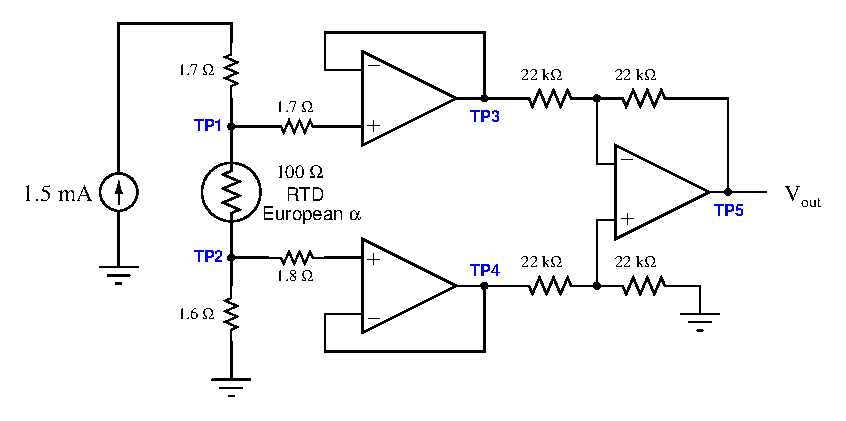
\includegraphics[width=15.5cm]{i00652x01.eps}$$

\begin{itemize}
\item{} Spenning ved TP1 ($V_{TP1}$), med RTD på 0$^{o}$ C = \underbar{\hskip 50pt} V
\vskip 5pt
\item{} Spenning ved TP2 ($V_{TP2}$), med RTD på 10$^{o}$ F = \underbar{\hskip 50pt} V
\vskip 5pt
\item{} Spenning ved TP3 ($V_{TP3}$), med RTD på 12$^{o}$ C = \underbar{\hskip 50pt} V
\vskip 5pt
\item{} Spenning ved TP5 ($V_{TP5}$), med RTD på -20$^{o}$ C = \underbar{\hskip 50pt} V
\end{itemize}

\underbar{file i00652no}
%(END_QUESTION)





%(BEGIN_ANSWER)

Husk disse forenklede antakelsene for op-amp-kretser med negativ tilbakekobling:

\begin{itemize}
\item{} Negativ tilbakekobling vil tvinge utgangsspenningen til den verdien som er nødvendig for å holde differensiell inngangsspenning lik null.
\item{} Inngangsterminalene på op-ampene trekker neglisjerbar strøm.
\end{itemize}

Spenningene ved TP1 og TP2 (med referanse til jord) kan beregnes enkelt ved å evaluere spenningsfall i serie-RTD-kretsen. Spenningen ved TP3 med referanse til jord vil være identisk med den ved TP1, siden øvre op-amp fungerer som en spenningsfølger. TP5 er utgangen fra denne differensialforsterkerkretsen, og representerer forskjellen mellom potensialene målt ved inngangene TP1 og TP2 (altså spenningsfallet over RTD-en). Grunnen til at utgangsspenningen er negativ (med hensyn til jord), er at differensialforsterkerens ikke-inverterende inngang ser lavere spenning enn den inverterende inngangen.

\vskip 10pt

For hver spenningsberegning må du bruke en RTD-tabell for å finne riktige RTD-motstandsverdier. Selv om det er mulig å bruke en formel for å tilnærme RTD-motstand basert på temperatur, gir tabell mer nøyaktige svar fordi tabellen tar hensyn til RTD-ens ikke-linearitet, mens formelen antar perfekt lineær karakteristikk.

\vskip 10pt

\begin{itemize}
\item{} Spenning ved TP1 ($V_{TP1}$), med RTD på 0$^{o}$ C ($R_{RTD}$ = 100.0 $\Omega$) = \underbar{\bf 0.1524} V
\vskip 5pt
\item{} Spenning ved TP2 ($V_{TP2}$), med RTD på 10$^{o}$ F ($R_{RTD}$ = 95.21 $\Omega$) = \underbar{\bf 0.0024} V ({\bf 2.4} mV)
\vskip 5pt
\item{} Spenning ved TP3 ($V_{TP3}$), med RTD på 12$^{o}$ C ($R_{RTD}$ = 104.68 $\Omega$) = \underbar{\bf 0.1594} V
\vskip 5pt
\item{} Spenning ved TP5 ($V_{TP5}$), med RTD på -20$^{o}$ C ($R_{RTD}$ = 92.16 $\Omega$) = \underbar{\bf -0.1382} V
\end{itemize}

%(END_ANSWER)





%(BEGIN_NOTES)


%INDEX% Måling, temperatur: RTD (4-leder med kabelmotstand)

%(END_NOTES)
